\documentclass[12pt]{report}
\usepackage{amsthm, amssymb}
\usepackage{geometry}
\geometry{legalpaper, margin=1in}
\usepackage{amsmath}
\usepackage{enumitem}

\newtheorem*{remark}{Remark}
\newtheorem{theorem}{Theorem}
\newtheorem{corollary}{Corollary}[theorem]
\newtheorem{lemma}[theorem]{Lemma}
\newtheorem*{defi}{Definition}
\newtheorem{ex}{Example}
\usepackage{xcolor}
\usepackage{graphicx}

\newcommand{\R}{\mathbb{R}^2}
\newcommand{\x}{\mathbf{x}}
\newcommand{\y}{\mathbf{y}}
\newcommand{\inv}{^{-1}}

\title{Topology HW 8}
\author{Ben Kallus}
\date{Due Friday, April 9, 2021}

\begin{document}

\maketitle

\newpage\noindent\textbf{1)} Let $X = [0,1] \times [0,1]$. Let $X^*$ consist of two types of subsets:

\medskip\textbf{1)} Sets consisting of a single point $\{(x,y)\}$ where $0 < x < 1, 0 \leq y \leq 1.$

\medskip\textbf{2)} Sets consisting of pairs of points $\{(0,y), (1,1-y)\}$ where $0 \leq y \leq 1.$

\begin{center}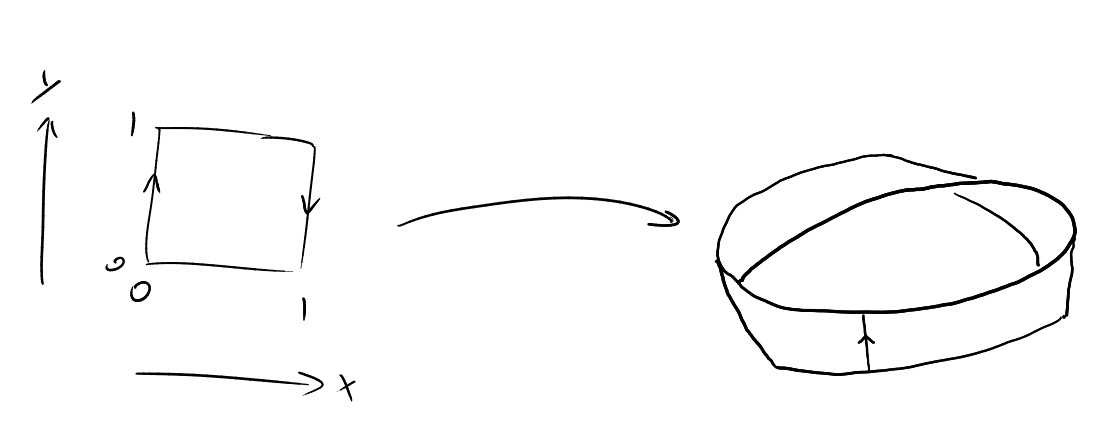
\includegraphics[scale=.5]{pic1.png}

The M\"obius strip.\end{center}

\newpage\noindent\textbf{2)} Let $X=[0,1] \times[0,1].$ Let $X^*$ consist of three types of subsets:

\medskip\textbf{1)} Sets consisting of a single point $\{(x,y)\}$ where $0 \leq x \leq 1$, $0 \leq y \leq 1$.

\medskip\textbf{2)} Sets consisting of pairs of point $\{(0,y),(1,1-y)\}$ where $0 \leq y \leq 1$.

\medskip\textbf{3)} Sets consisting of pairs of points $\{(x,0),(1-x,1)\}$ where $0 < x < 1$.

\begin{center}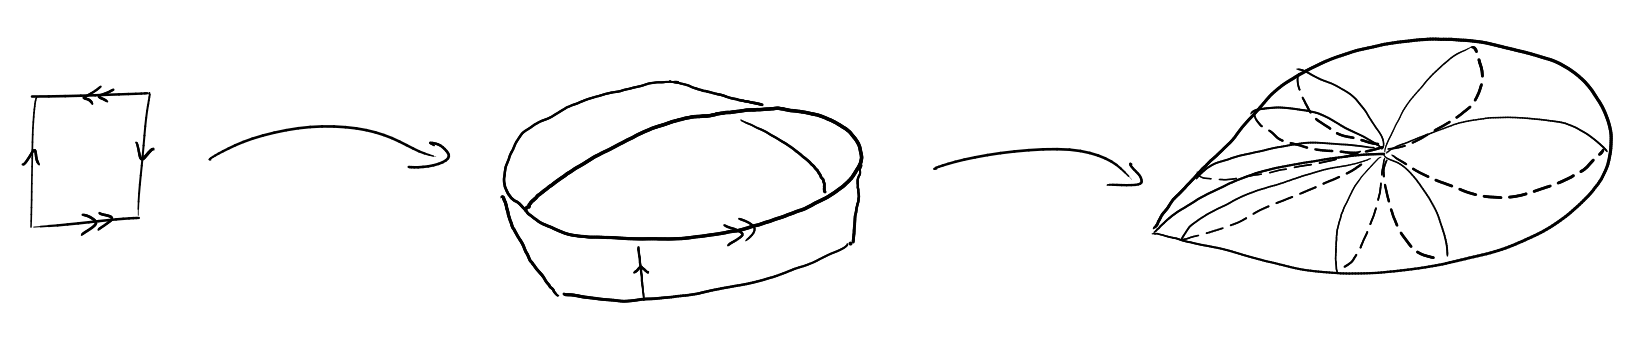
\includegraphics[scale=.4]{pic2.png}

The cross-cap.\end{center}

\newpage\noindent\textbf{3)} Proposition: If $f: X \to Y$ is a homeomorphism and $A \subseteq X$, then $(X \setminus A)$ is homeomorphic to $(Y \setminus f(A))$ with the subspace topologies from $X$ and $Y$.
\begin{proof}
    Let $X, Y$ be topological spaces.
    Let $f: X \to Y$ be a homeomorphism.
    Let $A \subseteq X$.

    By Theorem 18.2, $f|_{X \setminus A}: (X \setminus A) \to Y \setminus f(A)$ is continuous.
    Because $f$ is injective, $f|_{X \setminus A}$ must also be injective.
    Because $f$ is bijective, $f|_{X \setminus A}$ is onto $Y \setminus f(A)$.
    Thus, $f|_{X \setminus A}: (X \setminus A) \to (Y \setminus f(A))$ is a continuous bijection.

    By Theorem 18.2, $f\inv|{Y \setminus f(A)} : (Y \setminus f(A)) \to (X \setminus A)$ is continuous.
    Because $f\inv$ is injective, $f\inv|_{Y \setminus f(A)}$ must also be injective.
    Because $f\inv$ is bijective, $f\inv|_{Y \setminus f(A)}$ is onto $X \setminus A$.
    Thus, $f\inv|_{Y \setminus f(A)}: (Y \setminus f(A)) \to (X \setminus A)$ is a continuous bijection.

    Thus, $f|_{X \setminus A}$ is a homeomorphism, so $X \setminus A$ is homeomorphic to $Y \setminus f(A)$.
\end{proof}

\newpage\noindent\textbf{4)} Proposition: A topological space $X$ is connected if and only if the only subsets of $X$ that are clopen are $\emptyset$ and $X$.
\begin{proof}
    Suppose $A \subseteq X$ is both open and closed in $X$ such that $A \neq \emptyset$ and $A \neq X$.
    Thus, $X \setminus A$ is open in $X$ and since $A \neq X$ we have $X \setminus A$ is nonempty.
    Note $A \cup X \setminus A = X$.
    Therefore, $A$ and $X \setminus A$ is a separation of $X$.
    Thus, if $X$ is connected, then the only subsets of $X$ that are clopen are $\emptyset$ and $X$.

    Conversely, suppose that the only subsets of $X$ that are clopen are $\emptyset$ and $X$.
    Suppose, toward a contradiction, that $X$ has a separation $U,V$.
    Note that $U,V$ are therefore open in $X$.
    Then, $X \setminus U = V$.
    Thus, $U$ is closed in $X$.
    Therefore, $U$ is clopen in $X$, which contradicts our initial supposition.
    Thus, $X$ has no separation, so $X$ is connected.
\end{proof}


\end{document}
